%----------------------------------------------------------------------------------------
%    PACKAGES AND THEMES
%----------------------------------------------------------------------------------------

\documentclass[aspectratio=169,xcolor=dvipsnames]{beamer}
\usetheme{SimpleDarkBlue}

\usepackage{hyperref}
\usepackage{graphicx} % Allows including images
\usepackage{booktabs} % Allows the use of \toprule, \midrule and \bottomrule in tables

\usepackage{fontspec}
\usepackage{luatexja}

\usepackage{appendixnumberbeamer}

\setmainfont{Alegreya Sans Light}[
  ItalicFont={* Italic},
  BoldFont={Alegreya Sans Medium},
  BoldItalicFont={Alegreya Sans Medium Italic}]
\setsansfont{Alegreya Sans Light}[
  ItalicFont={* Italic},
  BoldFont={Alegreya Sans Medium},
  BoldItalicFont={Alegreya Sans Medium Italic}]

% ------------ %
% beamerbutton %
% ------------ %
\newcommand{\goto}[2]{\hyperlink{#2}{\beamergotobutton{#1}}}
\newcommand{\return}[2]{\hyperlink{#2}{\beamerreturnbutton{#1}}}
\newcommand{\extgoto}[2]{\href{#2}{\beamergotobutton{#1}}}

% % --------------------------- %
% % Section title page with toc %
% % --------------------------- %
% \setbeamertemplate{subsection page}{%
%     \usebeamertemplate*{section page}
% }
% \setbeamertemplate{section in toc}[square]
% \setbeamertemplate{subsection in toc}[square]
% \AtBeginSection[]{
% % \sepframe
% \begin{frame}[noframenumbering]{Outline}
%     % \tableofcontents[currentsection]
%     \tableofcontents[currentsection, currentsubsection]
% \end{frame}
% }
% \AtBeginSubsection[]{
%   \begin{frame}[noframenumbering]{Outline}
%     \tableofcontents[currentsection, currentsubsection]
%   \end{frame}
% }

% ------------------------------------ %
% Section title page with Huge bf text %
% ------------------------------------ %
\AtBeginSection[]{
  \begin{frame}[noframenumbering, plain]
    \Huge{\centerline{\textbf{\insertsection}}}
  \end{frame}
}

%%% automatically add spaces into enumerate and itemize environment
\let\tempone\itemize
\let\temptwo\enditemize
\renewenvironment{itemize}{\tempone\addtolength{\itemsep}{\fill}}{\temptwo}
\let\tempa\enumerate
\let\tempb\endenumerate
\renewenvironment{enumerate}{\tempa\addtolength{\itemsep}{\fill}}{\tempb}

%%=============================================================
%%  FOOTLINE TEMPLATE
%%=============================================================

% % --- Footline depends on onesec option: show only current section or full bar ---
% \if@Optiononesec
% % Minimalist footline: only section name and frame number
% \defbeamertemplate*{footline}{shadow theme}{%
%     \leavevmode\hbox{%
%         \hypersetup{linkcolor=white,urlcolor=white,citecolor=white}
%         \begin{beamercolorbox}[wd=1.01\paperwidth, ht=2.5ex, dp=1.125ex, leftskip=.3cm plus1fil, rightskip=0.3cm]{author in head/foot}%
%             \insertshorttitle \insertsection \hfill \insertframenumber \ / \ \inserttotalframenumber%
%         \end{beamercolorbox}%
%     }%
% }
% \else
% % Standard footline: section bar and frame number
\defbeamertemplate*{footline}{shadow theme}{%
    \leavevmode\hbox{%
        \hypersetup{linkcolor=white,urlcolor=white,citecolor=white}
        \begin{beamercolorbox}[wd=1.02\paperwidth, ht=2.5ex, dp=1.125ex, leftskip=.3cm plus1fil, rightskip=0.3cm]{author in head/foot}%
            \insertsectionnavigationhorizontal{.80\textwidth}{}{} \hspace{.3cm} \hfill \#\ \insertframenumber \ / \ \inserttotalframenumber%
        \end{beamercolorbox}%
    }%
}
% \fi

% --- Activate the custom footline ---
\setbeamertemplate{footline}[shadow theme]


%----------------------------------------------------------------------------------------
%    TITLE PAGE
%----------------------------------------------------------------------------------------

% \title[]{}
% \author{ Hui-Jun Chen\inst{1}
% \and Min Fang\inst{2}
% \and Po-Hsuan Hsu\inst{1}
% \and Chi-Yang Tsou\inst{3}
% \institute[]{
%     \inst{1} National Tsing Hua University \and
%     \inst{2} University of Florida \and
%     \inst{3} University of Manchester \and
%     }\vspace{2pt}
% \date{\today} % Date, can be changed to a custom date



\title[Lecture 4]{Graduate Macro Sequence:\\ One-Side Labor Search Model}
\author[Hui-Jun Chen]{Hui-Jun Chen}
\institute[]{National Tsing Hua University\\ Department of Economics}
\date{\today}

%----------------------------------------------------------------------------------------
%    PRESENTATION SLIDES
%----------------------------------------------------------------------------------------

\begin{document}

% \setbeamercovered{transparent}
%------------------------------------------------
\begin{frame}[plain,noframenumbering]
    % Print the title page as the first slide
    \titlepage
\end{frame}

%========================================================================================
% \section{One-Sided Search (McCall 1970)}
% \label{sec:OneSided_Search_McCall}
%========================================================================================

\begin{frame}{One-Sided search [McCall (1970)]}
\label{slide:McCall_01}
\small
decision maker = unemployed worker
\begin{itemize}
    \item infinitely lived and risk neutral
    \item no borrowing/lending
    \item no aggregate uncertainty
    \item lifetime utility $\sum_{t=0}^{\infty}\beta^t u(c_t)$, where $u(c_t)=c_t$
    \item One i.i.d.\ wage offer $w$ drawn each period while unemployed
    \item $w\sim F(w)$ defined on $[0,B]$, with $B\in\mathbb{R}_+$
    \item Accept $\rightarrow$ get $w$ each period forever, starting now
    \item Reject $\rightarrow$ get $c$ (UI insurance, etc) now; get new draw next period
\end{itemize}
\end{frame}

\begin{frame}{One-Sided search [McCall (1970)]}
\label{slide:McCall_02}
\small
unemployed worker's problem
\begin{itemize}
    \item define $v(w)$ as expected lifetime utility value of receiving offer $w$
    \item simple recursive formulation of problem:
    \[
        v(w)=\max\{V^{accept}(w),\,V^{reject}\}
    \]
    \[
        V^{accept}(w)=\sum_{t=0}^{\infty}\beta^t w=\frac{w}{1-\beta}
        \qquad
        V^{reject}=c+\beta\int_0^B v(w')F(dw')
    \]
    \item consolidated value function for an unemployed worker:
    \[
        v(w)=\max\left\{\frac{w}{1-\beta},\;c+\beta\int_0^B v(w')F(dw')\right\}
    \]
\end{itemize}
\end{frame}

\begin{frame}{One-Sided search [McCall (1970)]}
\label{slide:McCall_03}
\small
Value for a worker with offer $w$ in hand
\[
v(w)=\max\left\{\frac{w}{1-\beta},\;c+\beta\int_0^B v(w')F(dw')\right\}
\]
\begin{itemize}
    \item reservation wage:
    \[
        \frac{\bar w}{1-\beta}=c+\beta\int_0^B v(w')F(dw') \tag{1}
    \]
    \item restated functional equation:
    \[
        v(w)=
        \begin{cases}
            \displaystyle \frac{\bar w}{1-\beta}, & w\le \bar w \\
            \displaystyle \frac{w}{1-\beta}, & w\ge \bar w
        \end{cases}
        \tag{2}
    \]
    \item \emph{result 1:} reservation wage rises in unemployment compensation, $c$.
\end{itemize}
\end{frame}

\begin{frame}{First look at the reservation wage}
\label{slide:McCall_04}
\small
\begin{center}
    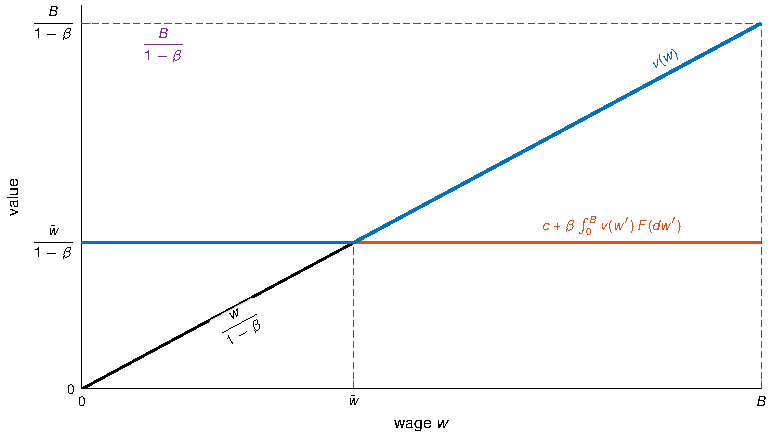
\includegraphics[width=0.75\textwidth]{figures/OneSidedSearch_TikZ_template_tex_pdf/fig_mccall_first_look_template.pdf}
\end{center}
\begin{itemize}
    \item \emph{result 1:} reservation wage rises in unemployment compensation, $c$.
    \item $v(w)$ also rises in $c$ [weakly].
\end{itemize}
\end{frame}

\section{First Characterization}
\label{sec:First_Characterization}

\begin{frame}{Characterizing the reservation wage (ver.\ 1)}
\label{slide:McCall_05}
\small
\[
\frac{\bar w}{1-\beta}=c+\beta\int_0^B v(w')F(dw')
\qquad\text{with}\qquad
v(w)=
\begin{cases}
\displaystyle \frac{\bar w}{1-\beta}, & w\le\bar w\\
\displaystyle \frac{w}{1-\beta}, & w\ge\bar w
\end{cases}
\]
\[
\frac{\bar w}{1-\beta}
= c+\beta\int_0^{\bar w}\frac{\bar w}{1-\beta}F(dw')
+\beta\int_{\bar w}^{B}\frac{w'}{1-\beta}F(dw')
\]
\[
\frac{\bar w}{1-\beta}
= c+\frac{\beta}{1-\beta}\bar w
+\frac{\beta}{1-\beta}\int_{\bar w}^{B}(w'-\bar w)F(dw')
\]
\[
\bar w-c=\frac{\beta}{1-\beta}\int_{\bar w}^{B}(w'-\bar w)F(dw') \tag{3}
\]
\end{frame}

\begin{frame}{Graphing the reservation wage (ver.\ 1)}
\label{slide:McCall_06}
\small
\[
\bar w-c=\frac{\beta}{1-\beta}\int_{\bar w}^{B}(w'-\bar w)F(dw') \tag{3}
\]
reservation wage solves $w-c=h(w)$, where
\[
h(w)\equiv \frac{\beta}{1-\beta}\int_{w}^{B}(w'-w)F(dw') \tag{4}
\]
\[
h(0)\equiv \frac{\beta}{1-\beta}\int_0^B (w')F(dw')=\frac{\beta}{1-\beta}Ew
\qquad
h(B)\equiv \frac{\beta}{1-\beta}\int_B^B (w'-B)F(dw')=0
\]
\end{frame}

\begin{frame}{Graphing the reservation wage (ver.\ 1)}
\label{slide:McCall_07}
\small
res.\ wage solves $w-c=h(w)$, with $h(w)\equiv \frac{\beta}{1-\beta}\int_{w}^{B}(w'-w)F(dw')$

\vspace{0.4em}
recall Leibniz:
\[
\frac{\partial}{\partial z}\left[\int_{a(z)}^{b(z)} f(x,z)\,dx\right]
=\int_{a(z)}^{b(z)}\left[\frac{\partial f(x,z)}{\partial z}\right]dx
+b'(z)f(b(z),z)-a'(z)f(a(z),z)
\]
this application: $[w'-w]F'(w')dw'$ is $f(x,z)dx$ and $w$ is $z$ and $w'$ is $x$
\[
h'(w)=\frac{\beta}{1-\beta}\left[\int_{w}^{B} -F'(w')\,dw' +[0\cdot(B-w)]-[1\cdot(w-w)]\right]
\]
\[
h'(w)=-\frac{\beta}{1-\beta}[F(B)-F(w)]=-\frac{\beta}{1-\beta}[1-F(w)]<0 \quad\text{for } w<B
\]
\[
h''(w)=\frac{\beta}{1-\beta}F'(w)>0 \quad\text{for } w<B
\]
\begin{itemize}
    \item RHS of wage equation, $w-c=h(w)$, is downward sloping and convex
\end{itemize}
\end{frame}

\begin{frame}{Second look at the reservation wage}
\label{slide:McCall_08}
\small
\begin{center}
    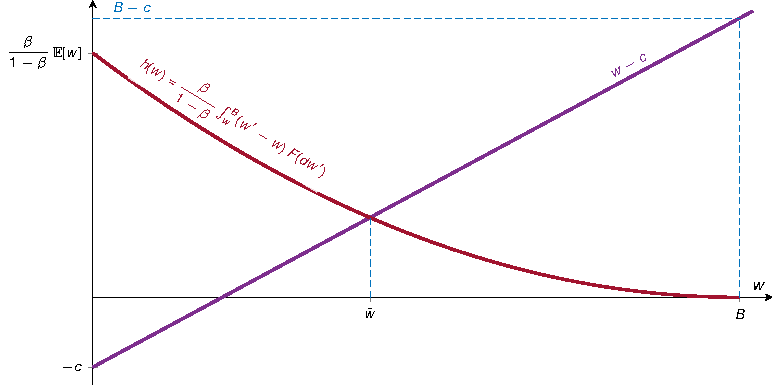
\includegraphics[width=0.78\textwidth]{figures/OneSidedSearch_TikZ_template_tex_pdf/fig_mccall_second_look_template.pdf}
\end{center}
\begin{itemize}
    \item higher $\beta$ pivots $h(w)$ upward, with no effect on LHS.
    \item \emph{result 2:} reservation wage rises with patience, $\beta$.
\end{itemize}
\end{frame}

\begin{frame}{Mean-Preserving Spread}
\label{slide:McCall_09}
\small
\emph{Definition Part A:} Let $F(x)$ and $H(x)$ be two distributions on $x\in[0,B]$ with the same mean...

\vspace{0.4em}
\[
Ex=\int_0^B xF(dx)=\int_0^B xH(dx)
\]
recall $\int_a^b u\,dv = uv\big|_a^b - \int_a^b v\,du$ and set $u=x$, $dv=F(dx)$:
\[
\int_0^B xF(dx)=xF(x)\big|_0^B-\int_0^B F(x)\,dx = B-\int_0^B F(x)\,dx
\]
\[
\text{Common Mean:}\quad Ex = B-\int_0^B F(x)\,dx = B-\int_0^B H(x)\,dx
\]
\[
\text{Common Mean:}\quad \int_0^B [F(x)-H(x)]\,dx = 0 \tag{5a}
\]
\end{frame}

\begin{frame}{Mean-Preserving Spread}
\label{slide:McCall_10}
\small
\emph{Definition Part B:} And let $F$ and $H$ have the single crossing property...

\vspace{0.4em}
\[
\text{Single Crossing: }\ \exists\,\hat x\in(0,B)\ \text{ such that }\
F(x)-H(x)\ \begin{cases}
\ge 0 & \text{at } x\le \hat x\\
\le 0 & \text{at } x\ge \hat x
\end{cases}
\tag{5b}
\]

\vspace{0.2em}
\emph{Definition Part C:} Then $F$ is a Mean-Preserving Spread of $H$.

\begin{itemize}
    \item combining (5b) and (5a):
    \[
        0=\int_0^B [F(x)-H(x)]dx
        =\int_0^{\hat x}[F(x)-H(x)]dx+\int_{\hat x}^{B}[F(x)-H(x)]dx
    \]
\end{itemize}

\textbf{Implication:} If $F$ is a Mean-Preserving Spread of $H$, then:
\[
\int_0^{y}[F(x)-H(x)]dx\ge 0
\quad \forall y\in[0,B]
\tag{5c}
\]
\end{frame}

\section{Second Characterization}
\label{sec:Second_Characterization}


\begin{frame}{Characterizing the reservation wage (ver.\ 2)}
\label{slide:McCall_11}
\small
\begin{itemize}
    \item an alternative expression, beginning with equation (3)
\end{itemize}
\[
\bar w-c=\frac{\beta}{1-\beta}\int_{\bar w}^{B}(w'-\bar w)F(dw')
+\frac{\beta}{1-\beta}\int_0^{\bar w}(w'-\bar w)F(dw')
-\frac{\beta}{1-\beta}\int_0^{\bar w}(w'-\bar w)F(dw')
\]
\[
\bar w-c=\frac{\beta}{1-\beta}\int_{0}^{B}(w'-\bar w)F(dw')
-\frac{\beta}{1-\beta}\int_0^{\bar w}(w'-\bar w)F(dw')
\]
\[
\bar w-(1-\beta)c
=\beta\int_0^{B} w'F(dw')-\beta\int_0^{\bar w}(w'-\bar w)F(dw')
\]
\[
\bar w-c=\beta(Ew-c)-\beta\int_0^{\bar w}(w'-\bar w)F(dw') \tag{**}
\]
\end{frame}

\begin{frame}{Characterizing the reservation wage (ver.\ 2)}
\label{slide:McCall_12}
\small
\begin{itemize}
    \item so far:
    \[
        \bar w-c=\beta(Ew-c)-\beta\int_0^{\bar w}(w'-\bar w)F(dw') \tag{**}
    \]
    \item $\int_a^b u\,dv=uv\big|_a^b-\int_a^b v\,du$. Set $u=[w'-\bar w]$, $dv=F'(w')dw'$.
\end{itemize}
\[
\int_0^{\bar w}(w'-\bar w)F(dw')
=(w'-\bar w)F(w')\big|_0^{\bar w}-\int_0^{\bar w}F(w')dw'
=-\int_0^{\bar w}F(w')dw'
\]
\begin{itemize}
    \item replacing the integral in (**), we can identify $\bar w$ via:
\end{itemize}
\[
\bar w-c=\beta(Ew-c)+\beta\int_0^{\bar w}F(w')dw' \tag{6}
\]
\end{frame}

\begin{frame}{Graphing the reservation wage (ver.\ 2)}
\label{slide:McCall_13}
\small
\begin{itemize}
    \item From (6), we know $\bar w$ is the $w$ satisfying:
    \[
        w-c=\beta(Ew-c)+\beta\int_0^{w}F(w')dw'
    \]
    \item LHS is linear, starts at $-c$, with slope 1.
    \item Term 1 of RHS is a constant $\ge -c$.
    \item Term 2 of RHS is $g(w)\equiv \beta\int_0^{w}F(w')dw'$.
    \item $g(0)=0$. \quad $g'(w)=\beta F(w)\ge 0$. \quad $g''(w)=\beta F'(w)\ge 0$.
\end{itemize}

\vspace{0.4em}
\hrule
\footnotesize
Leibniz Rule:
\[
\frac{\partial}{\partial z}\left[\int_{a(z)}^{b(z)} f(x,z)\,dx\right]
=\int_{a(z)}^{b(z)}\left[\frac{\partial f(x,z)}{\partial z}\right]dx
+b'(z)f(b(z),z)-a'(z)f(a(z),z)
\]
\[
g'(w)=\beta\frac{\partial}{\partial w}\left[\int_0^w F(w')dw'\right]
=\beta\left[\int_0^w \frac{\partial F(w')}{\partial w}\,dw' + 1\cdot F(w)-0\cdot F(0)\right]
=\beta F(w)
\]
\end{frame}

\begin{frame}{Graph of Equation (6)}
\label{slide:McCall_14}
\small
\begin{center}
    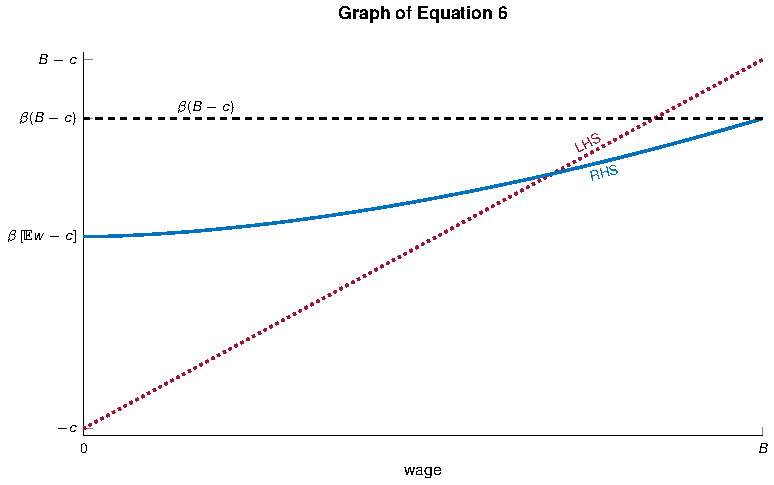
\includegraphics[width=0.80\textwidth]{figures/OneSidedSearch_TikZ_template_tex_pdf/fig_mccall_graph_eq6_template.pdf}
\end{center}
\end{frame}

\begin{frame}{Graphing the reservation wage (ver.\ 2)}
\label{slide:McCall_15}
\small
$\bar w$ is the $w$ satisfying: \quad $w-c=\beta(Ew-c)+\beta\int_0^{w}F(w')dw'$.

\vspace{0.5em}
\textbf{What if $F$ is replaced by $G$, a Mean Preserving Spread of $F$?}
\begin{itemize}
    \item Linear LHS unchanged. \quad Constant Term 1 of RHS unchanged.
    \item Increasing, convex Term 2 of RHS,
    \[
        g_F(w)\equiv \beta\int_0^{w}F(w')dw',
        \quad\text{becomes}\quad
        g_G(w)\equiv \beta\int_0^{w}G(w')dw'.
    \]
    \item Prior results on Mean Preserving Spreads tell us
    \[
        \int_0^{y}[G(w')-F(w')]dw' > 0
        \quad \forall y\in[0,B). \tag{5c}
    \]
    \item \emph{result 3:} reservation wage rises with a MPS on wage offers.
\end{itemize}
\end{frame}

\begin{frame}{Hazard and Unemployment Duration}
\label{slide:McCall_16}
\small
\textbf{A. Hazard:} Start-of-period employment probability (pre-$w$-draw)
\[
H_t=\Pr(accept)=1-\Pr(reject)=1-F(\bar w)
\]

\vspace{0.3em}
\textbf{B. Unemployment Spell of Duration $D=d$} occurs when $d-1$ offers are rejected and subsequent offer is accepted.\footnote{\scriptsize Given this definition (adopting the convention in the search literature), we identify immediate job acceptance as an unemployment spell of duration 1. Thus, unemployment durations run $d=1,2,\ldots$}

\vspace{0.2em}
\begin{itemize}
    \item $\Pr(D=1)=H_t$
    \item For $d>1$: $\Pr(D=d)=(1-H_t)(1-H_{t+1})\cdots(1-H_{t+d-2})\cdot H_{t+d-1}$
    \item All cases, $d\ge 1$:
    \[
        \Pr(D=d)=(1-H)^{d-1}\cdot H = [F(\bar w)]^{d-1}[1-F(\bar w)]
    \]
\end{itemize}
\end{frame}

\begin{frame}{Hazard and Unemployment Duration}
\label{slide:McCall_17}
\small
\textbf{A. Hazard:} Start-of-period employment probability (pre-$w$-draw)
\[
H_t=\Pr(accept)=1-\Pr(reject)=1-F(\bar w)
\]
\textbf{B. Unemployment Spell of Duration $D=d$} occurs when $d-1$ offers are rejected and subsequent offer is accepted.
\[
\Pr(D=d)=[F(\bar w)]^{d-1}[1-F(\bar w)],\quad \text{for all } d\ge 1
\]
\textbf{C. Expected Unemployment Duration:}
\[
ED=\sum_{d=1}^{\infty} d\cdot (1-H)^{d-1}\cdot H
\]
\end{frame}

\begin{frame}{Expected Unemployment Duration}
\label{slide:McCall_18}
\footnotesize
Expected Duration:
\[
ED=\sum_{d=1}^{\infty} d\cdot (1-H)^{d-1}\cdot H
\]

\hrule
\smallskip
A Handy Trick:
\[
\sum_{d=0}^{\infty}\Pr(D=d)=\sum_{d=0}^{\infty}(1-H)^d\cdot H \equiv 1.
\]
Differentiate w.r.t.\ $H$:
\[
\sum_{d=0}^{\infty} d(1-H)^{d-1}\cdot (-H)
+\sum_{d=0}^{\infty}(1-H)^d =0
\]
\[
\Rightarrow\ \sum_{d=0}^{\infty} d(1-H)^{d-1}\cdot H = \frac{1}{1-(1-H)}
\quad [d=0\text{ contributes 0 on LHS}]
\]
\[
\Rightarrow\ \sum_{d=1}^{\infty} d(1-H)^{d-1}\cdot H = \frac{1}{H}
\]
\hrule
\smallskip
\textcolor{blue}{Expected Unemployment Duration:}\quad $ED=\dfrac{1}{H}=[1-F(\bar w)]^{-1}$.
\end{frame}

\begin{frame}{Influence of $c$ and $F(w)$ on Duration and Welfare}
\label{slide:McCall_19}
\small
\begin{itemize}
    \item Worker's optimal policy is a stationary reservation wage strategy, with reservation wage implicitly defined by (6).
    \[
        \bar w-c=\beta(Ew-c)+\beta\int_0^{\bar w}F(w')dw' \tag{6}
    \]
    \item Raised $c$ or MPS of $F\Rightarrow \bar w\uparrow \Rightarrow F(\bar w)\uparrow \Rightarrow H\downarrow \Rightarrow ED\uparrow$
    \item Longer unemployment duration does NOT imply the worker is hurt by $c\uparrow$ or MPS in wage offers. Quite the converse.
    \[
        Ev=\frac{\bar w}{1-\beta}F(\bar w)+\int_{\bar w}^{B}\frac{w}{1-\beta}F(dw)
    \]
    \item \emph{Unemployment is voluntary.} Higher UI compensation or higher probability of right-tail offers (with protection from left tail) make the worker choosier, raising $\bar w$, unemployment duration, and welfare.
\end{itemize}
\end{frame}

\begin{frame}{Simple extensions (some you will do)}
\label{slide:McCall_20}
\small
\begin{itemize}
    \item same basic reservation wage analysis applies for a firm choosing whether to accept/reject wage bids (period profits falling in $w$).
    \item same basic reservation wage analysis applies to the case of multiple offers in a period (costlessly observed)
    \item analysis also extends to allow nonzero per-period probability of receiving no offer (or allowing worker to choose search intensity)
    \item allowing recall has no effect on policy or reservation wage
    \item if quits are allowed, but they incur a 1-period unemployment penalty (permitting no on-the-job-search), option is never exercised
    \item if worker can be fired in any period with probability $\alpha\in(0,1)$, same policy applies, but with lower $\bar w$...
\end{itemize}
\end{frame}

\begin{frame}{Exogenous firing extension}
\label{slide:McCall_21}
\small
\begin{itemize}
    \item With probability $\alpha\in(0,1)$, worker is fired. When fired, worker must sit unemployed for 1 period; thereafter, offers begin.
    \item Let $\hat v^{E}(w)$ be the value to a worker of being employed with wage $w$.
    Value of receiving wage offer $w$ is then:
\end{itemize}
\[
\hat v(w)=\max\left\{\hat v^{E}(w),\;c+\beta\int_0^B \hat v(w')F(dw')\right\} \tag{A}
\]
\[
\text{where}\qquad
\hat v^{E}(w)=w+\beta(1-\alpha)\hat v^{E}(w)+\beta\alpha\left[c+\beta\int_0^B \hat v(w')F(dw')\right] \tag{B}
\]
\begin{itemize}
    \item Rearrange (B):
\end{itemize}
\[
\hat v^{E}(w)=\frac{1}{1-\beta(1-\alpha)}\left[w+\beta\alpha\left(c+\beta\int_0^B \hat v(w')F(dw')\right)\right] \tag{C}
\]
\end{frame}

\begin{frame}{Exogenous firing extension part 2}
\label{slide:McCall_22}
\small
\[
\hat v(w)=\max\left\{\hat v^{E}(w),\;c+\beta\int_0^B \hat v(w')F(dw')\right\} \tag{A}
\]
\[
\text{where}\qquad
\hat v^{E}(w)=\frac{1}{1-\beta(1-\alpha)}\left[w+\beta\alpha\left(c+\beta\int_0^B \hat v(w')F(dw')\right)\right] \tag{C}
\]
\begin{itemize}
    \item Put (C) in (A), defining $E\hat v \equiv \int_0^B \hat v(w)F(dw)$:
\end{itemize}
\[
\hat v(w)=\max\left\{
\frac{w+\beta\alpha\left[c+\beta E\hat v\right]}{1-\beta(1-\alpha)},\;
c+\beta E\hat v
\right\}
\]
\begin{itemize}
    \item Reservation wage solves:
\end{itemize}
\[
\bar w+\beta\alpha\left[c+\beta E\hat v\right]
=
[1-\beta(1-\alpha)]c+[1-\beta(1-\alpha)]\beta E\hat v
\]
\end{frame}

\begin{frame}{Exogenous firing extension part 3}
\label{slide:McCall_23}
\small
\begin{itemize}
    \item Reservation wage solves:
\end{itemize}
\[
\bar w+\beta\alpha\left[c+\beta E\hat v\right]
=
[1-\beta(1-\alpha)]c+[1-\beta(1-\alpha)]\beta E\hat v
\]
\[
\Rightarrow\quad \bar w=(1-\beta)\left[c+\beta E\hat v\right]
\]
\[
\frac{\bar w}{1-\beta}=c+\beta\int_0^B \hat v(w)F(dw) \tag{D}
\]
\begin{itemize}
    \item Compare (D) to (1). Unaltered reservation wage policy...
    \item But, since $\hat v(w)<v(w)$, the critical $\bar w$ is lower with firing.
    \item Why? \emph{Possibility of being fired lowers expected return to search.}
\end{itemize}
\end{frame}

\begin{frame}{Firing probability and the reservation wage}
\label{slide:McCall_24}
\small
\begin{center}
    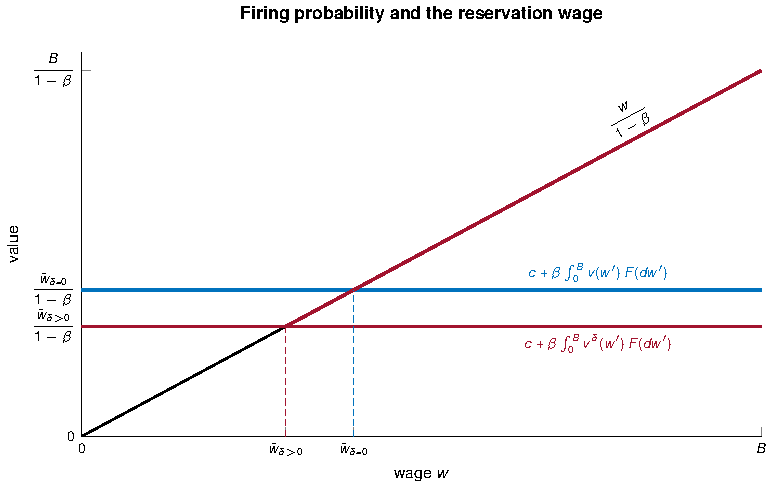
\includegraphics[width=0.65\textwidth]{figures/OneSidedSearch_TikZ_template_tex_pdf/fig_mccall_firing_prob_template.pdf}
\end{center}
\begin{itemize}
    \item both welfare and the reservation wage fall with firing probability
\end{itemize}
\end{frame}

\end{document}
